\section{Task 1}
Să se creeze baza de date calculatoare (tabelele, constrîngerile de integritate), utilizînd limbajul Transact-SQL.

\begin{figure}[H]
	\centering
		\minipage{0.48\textwidth}
		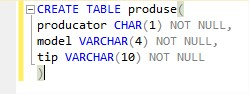
\includegraphics[width=\linewidth]{screens/1.jpg}
		\caption*{Figure 1: Produse table creation}
		\label{}
	\endminipage\hfill
		\minipage{0.48\textwidth}%
		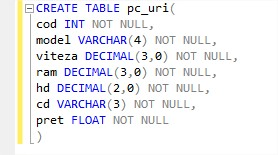
\includegraphics[width=\linewidth]{screens/2.jpg}
		\caption*{Figure 2: PC\_uri table creation}
	\endminipage
\end{figure}

\begin{figure}[H]
	\centering
		\minipage{0.48\textwidth}
		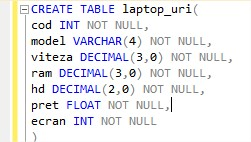
\includegraphics[width=\linewidth]{screens/3.jpg}
		\caption*{Figure 3: Laptop\_uri table creation}
		\label{}
	\endminipage\hfill
		\minipage{0.48\textwidth}%
		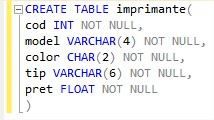
\includegraphics[width=\linewidth]{screens/4.jpg}
		\caption*{Figure 4: Imprimante table creation}
	\endminipage
\end{figure}

\begin{figure}[H]
	\centering
		\minipage{0.48\textwidth}
		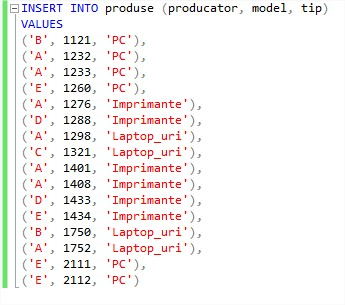
\includegraphics[width=\linewidth]{screens/5.jpg}
		\caption*{Figure 5: Fill produse table}
		\label{}
	\endminipage\hfill
		\minipage{0.48\textwidth}%
		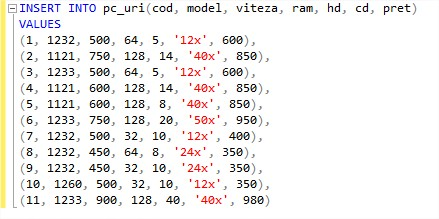
\includegraphics[width=\linewidth]{screens/6.jpg}
		\caption*{Figure 6: Fill pc\_uri table}
	\endminipage
\end{figure}

\begin{figure}[H]
	\centering
		\minipage{0.48\textwidth}
		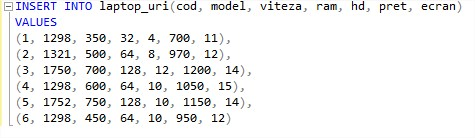
\includegraphics[width=\linewidth]{screens/7.jpg}
		\caption*{Figure 7: Fill laptop\_uri table}
		\label{}
	\endminipage\hfill
		\minipage{0.48\textwidth}%
		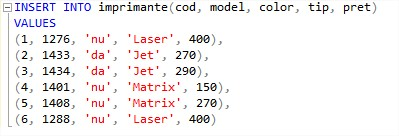
\includegraphics[width=\linewidth]{screens/8.jpg}
		\caption*{Figure 8: Fill imprimante table}
	\endminipage
\end{figure}



\section{Task 2}
Să se creeze tabelul imprimante\_stoc cu aceeași structură ca și tabelul imprimante. Să se însereze toate datele din tabelul imprimante în tablul imprimante\_stoc. Să se scrie, cu acest scop, un număr minimal de instrucțiuni. 

\begin{figure}[H]
	\centering
		\minipage{0.48\textwidth}
		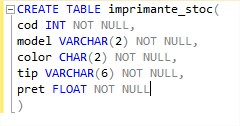
\includegraphics[width=\linewidth]{screens/9.jpg}
		\caption*{Figure 9: Creating the imprimante\_stoc table}
		\label{}
	\endminipage\hfill
		\minipage{0.48\textwidth}%
		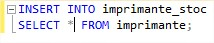
\includegraphics[width=\linewidth]{screens/10.jpg}
		\caption*{Figure 10: Insert the data from the imprimante table into the imprimante\_stoc table}
	\endminipage
\end{figure}
	
\section{Task 3}

Adăugați în tabelul pc\_uri modelul 444 cu codul 22, care are viteza procesorului 1200 și prețul 1350. Caracteristicile care lipsesc trebuie să fie completate cu valori implicite definite pentru coloanele respective. Pentru realizarea sarcinii cu succes trebuie să se modifice schema tabelului, utilizînd instructiunile DDL respective.

\begin{figure}[H]
	\centering
		\minipage{0.48\textwidth}
		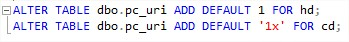
\includegraphics[width=\linewidth]{screens/13.jpg}
		\caption*{Figure 11: Add default data into table}
		\label{}
	\endminipage\hfill
		\minipage{0.48\textwidth}%
		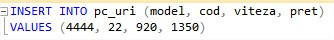
\includegraphics[width=\linewidth]{screens/14.jpg}
		\caption*{Figure 12: Inserting the data into the pc\_uri table}
	\endminipage
\end{figure}

\section{Task 4}
Pentru fiecare model de laptopuri, să se adauge o înregistrare în tabelul pc\_uri cu următoarele caracteristici: 
\begin{itemize}
	\item Cod: codul minimal al laptopului în grup + 30
	\item Model: numărul de model al laptopului + 100
	\item Viteza: citeza maximală a laptopului în grup
	\item Ram: capacitatea maximală a memoriei operative a laptopului în grup * 2
	\item Hd: capacitatea maximală a discului dur al laptopului în grup * 2
	\item Cd: valoare implicită
	\item Preț: prețul maximal al laptopului în grup, micșorat de 1.5 ori
\end{itemize}
	
\begin{figure}[H]
	\centering
		\minipage{0.48\textwidth}
		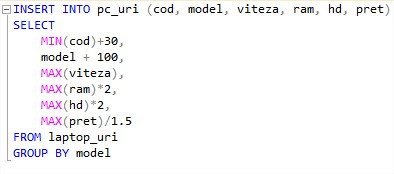
\includegraphics[width=\linewidth]{screens/16.jpg}
		\caption*{Figure 13: Inserting data into pc\_uri table}
		\label{}
	\endminipage\hfill
\end{figure}

\section{Task 6}
Să se scrie interogări de creare a indecșilor asupra tabelelor din baza de date calculatoare pentru a asigura o performanță sporită la executarea interogărilor SELECT din Lucrarea practică 4. Rezultatele optimizării să fie analizate în baza planurilor de execuție pînă și după crearea indecșilor.

CREATE INDEX i1 ON laptop\_uri (cod, model, viteza, ram, hd, pret, ecran);
	
\begin{figure}[H]
	\centering
		\minipage{0.48\textwidth}
		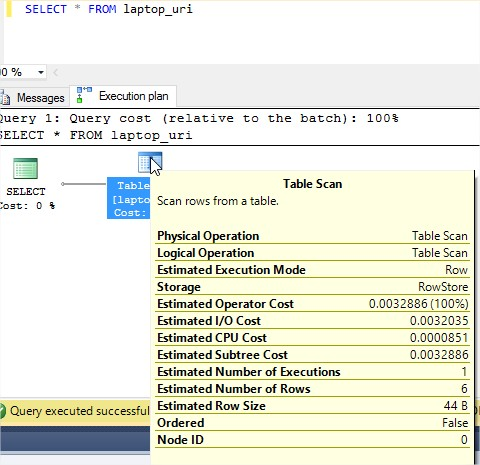
\includegraphics[width=\linewidth]{screens/19.jpg}
		\caption*{Figure 14: Execution plan for laptop\_uri}
		\label{}
	\endminipage\hfill
		\minipage{0.48\textwidth}%
		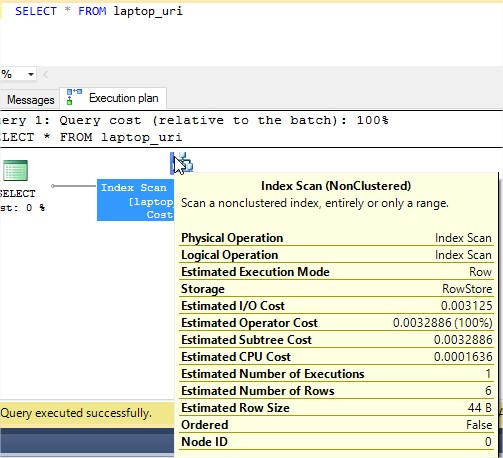
\includegraphics[width=\linewidth]{screens/20.jpg}
		\caption*{Figure 15: Result for laptop\_uri}
	\endminipage
\end{figure}
\bigskip